\documentclass[11pt]{article}

\usepackage[T1]{fontenc}
\usepackage{lmodern}
\usepackage[margin=1in]{geometry}
\usepackage{amsmath,amssymb}
\usepackage{graphicx}
\usepackage{booktabs}
\usepackage{caption}
\usepackage{enumitem}
\usepackage{microtype}
\usepackage{xcolor}
\usepackage[round]{natbib}
\usepackage[colorlinks=true,linkcolor=blue!50!black,citecolor=blue!50!black,urlcolor=blue!50!black]{hyperref}

\graphicspath{{../docs/figures/}}
\setlist{itemsep=2pt,topsep=4pt}

\newcommand{\code}[1]{\texttt{#1}}

\title{Pairs Trading, Tested Honestly:\\[2pt]
\large Cointegration Screens, Ornstein--Uhlenbeck Spreads, Kalman Hedge Ratios,\\
and a Walk-Forward Backtest on US Equities, 2019--2026}
\author{[Your Name]\\[2pt]
\small Code: \url{https://github.com/sashakrem/alpaca-pairs}}
\date{November 2026}

\begin{document}
\maketitle

\begin{abstract}
\noindent
Pairs trading bets that the gap between two related securities will close after it widens.
This paper tests whether the strategy still earns money on liquid US stocks and ETFs, using
daily data from the Alpaca market-data API (2016--2026). We screen pairs with Engle--Granger
cointegration tests, control the false discovery rate with the Benjamini--Hochberg procedure,
model the spread as an Ornstein--Uhlenbeck (OU) process, and check every pair on held-out
data with frozen parameters. A second screen tracks a time-varying hedge ratio with a Kalman
filter. We show that two common Kalman formulations find ``pairs'' in pure noise, and we
propose a returns-based model that tests the self-financing portfolio a trader would
actually hold. A walk-forward backtest with a one-day execution lag, per-side transaction
costs and short-borrow fees then trades the selected pairs year by year from 2019 to 2026.
Across 8{,}672 pair-years, 6.5\% look cointegrated at $p<0.05$, barely above the 5\% expected
by chance; after correction and out-of-sample validation, one survives. The distance-method
benchmark of \citet{gatev2006} earns a Sharpe ratio of $+0.16$ ($t=0.46$) before costs and
$-0.41$ at 5 basis points per side. The same code earns a Sharpe ratio of $+1.6$ on synthetic
markets with planted pairs, so the negative result reflects the market, not the
implementation. We close with open research questions and a roadmap of next steps.
\end{abstract}

\section{Introduction}

Some securities move together for economic reasons: two consumer-staples companies selling
similar products, two regional banks exposed to the same interest rates, two ETFs tracking
the same index. When the price gap between such securities widens beyond its usual range, a
pairs trader buys the laggard and shorts the leader. If the gap closes, the trade profits
regardless of the market's direction.

The idea is old and well studied. \citet{gatev2006} reported large excess returns for a
simple version over 1962--2002, and \citet{do2010} found that those profits largely vanished
after 2002. The practical difficulty is not writing a pairs strategy; it is avoiding the many
ways a backtest can fool its author. Three are central:
\begin{enumerate}
  \item \textbf{Multiple testing.} With $N$ securities there are $N(N-1)/2$ pairs. At a 5\%
        significance level, about 5\% of unrelated pairs pass any single test by chance.
  \item \textbf{Look-ahead bias.} Parameters estimated on the same data used to evaluate the
        strategy make it look better than it can be in practice.
  \item \textbf{Model flexibility.} Adaptive models, such as Kalman filters with drifting
        intercepts, can make any two series look related.
\end{enumerate}

This paper builds a pipeline designed around those three problems and asks a simple question:
\emph{after realistic costs, does pairs trading make money on liquid US equities from 2019
to 2026?} Our answer is no. The contribution is the care taken to reach that answer:
synthetic ground-truth validation, explicit false-discovery control, frozen out-of-sample
tests, a demonstration of two Kalman-filter traps, and a walk-forward backtest with trading
rules fixed before any results were seen.

\section{Background and related work}

\citet{engle1987} define two non-stationary series as \emph{cointegrated} if some linear
combination of them is stationary, and propose the two-step test used here: estimate the
combination by ordinary least squares, then test the residual for a unit root with the
augmented Dickey--Fuller (ADF) test \citep{dickey1979}. \citet{vidyamurthy2004} and
\citet{elliott2005} popularized cointegration and mean-reverting spread models for pairs
trading. The OU process \citep{uhlenbeck1930} is the standard continuous-time model of
mean reversion.

\citet{gatev2006} introduced the \emph{distance method}: match each stock with the one whose
normalized price path was closest over the past year, then trade divergences. It uses no
statistical test and is the common academic benchmark. \citet{do2010} documented its decline.

On the statistical side, \citet{benjamini1995} introduced false discovery rate (FDR) control,
which suits screening problems with many hypotheses. \citet{schwert1989} showed that unit-root
tests can over-reject in some settings. \citet{harvey2016} and \citet{bailey2014} argue that
financial research routinely understates the effect of multiple testing on reported Sharpe
ratios. The Kalman filter \citep{kalman1960} is widely used in practice to track time-varying
hedge ratios.

\section{Data}

Daily closing prices come from the Alpaca market-data API (\code{alpaca-py}), using the
consolidated SIP feed, adjusted for splits and dividends. Symbols missing more than 5\% of
trading days are dropped; remaining gaps are forward-filled. Prices are cached locally.

Pairs are searched only \emph{within} a sector, because an economic reason to co-move makes
a statistical relationship more credible and reduces the number of tests. Stages~1 and~2 use
five universes of ten large-cap stocks each (banks, energy, consumer staples, semiconductors,
utilities), plus a control set of near-identical instruments (GLD/IAU, SPY/IVV, GOOGL/GOOG,
EWA/EWC). The Stage~3 backtest uses six wider universes of twenty names that include mid caps
(banks, utilities, energy, REITs, consumer staples, country ETFs), about 120 symbols in total,
on the view that heavily traded mega-cap pairs are the most likely to have been arbitraged away.

\paragraph{Survivorship bias.} All universes are lists of companies that exist today.
Companies acquired or delisted during the sample (for example, regional banks that failed in
2023) are missing. This biases results \emph{upward}, which strengthens a negative finding.

\section{Methodology}

All prices are in logs. Let $y_t=\log Y_t$ and $x_t=\log X_t$.

\subsection{Cointegration screen (Stage 1)}

For each pair, the data are split at a date into a \emph{formation} period and a
\emph{holdout} period. On the formation period, the Engle--Granger test is run in both
directions ($y$ on $x$ and $x$ on $y$). Choosing the better direction is a second chance to
pass, so the smaller $p$-value is Bonferroni-corrected by doubling it. The hedge ratio
$\beta$ and offset $\alpha$ come from the regression
\begin{equation}
  y_t = \alpha + \beta x_t + s_t ,
\end{equation}
and the residual $s_t$ is the \emph{spread}.

\subsection{Multiple-testing control}

The direction-corrected $p$-values of all pairs in a universe are passed to the
Benjamini--Hochberg procedure at $q=0.05$. Sort the $m$ $p$-values
$p_{(1)}\le\dots\le p_{(m)}$; the adjusted values are
\begin{equation}
  \tilde p_{(i)} = \min_{k\ge i}\; \min\!\left(1,\, \frac{m\,p_{(k)}}{k}\right),
\end{equation}
and a pair is declared significant if $\tilde p \le q$. This bounds the expected share of
false discoveries among the pairs declared significant at about $q$.

\subsection{Ornstein--Uhlenbeck spread model}

The spread is modeled as
\begin{equation}
  dX_t = \theta(\mu - X_t)\,dt + \sigma\,dW_t ,
\end{equation}
where $\theta$ is the speed of mean reversion, $\mu$ the long-run mean and $\sigma$ the
volatility. Sampled at interval $\Delta t$, the process is exactly an AR(1):
\begin{equation}
  X_{t+1} = a + b X_t + \varepsilon_t,\qquad b=e^{-\theta\Delta t},\quad a=\mu(1-b),\quad
  \varepsilon_t\sim\mathcal N\!\left(0,\;\sigma^2\frac{1-b^2}{2\theta}\right).
\end{equation}
Ordinary least squares of $X_{t+1}$ on $X_t$ therefore gives the conditional
maximum-likelihood estimates by inverting these relations. If $b\notin(0,1)$ the series shows
no mean reversion and is rejected. Two derived quantities drive the strategy:
\begin{equation}
  \text{half-life} = \frac{\ln 2}{\theta},\qquad
  \sigma_{\infty} = \frac{\sigma}{\sqrt{2\theta}} ,
\end{equation}
where $\sigma_\infty$ is the standard deviation of the stationary distribution. The trading
signal is the z-score $z_t=(s_t-\mu)/\sigma_\infty$. Stage~1 requires a formation half-life
between 2 and 60 trading days.

The implementation also offers Euler--Maruyama simulation, whose AR coefficient is
$1-\theta\Delta t$ rather than $e^{-\theta\Delta t}$. A unit test confirms that fitting
Euler-simulated paths biases $\hat\theta$, increasingly so as $\theta\Delta t$ grows.

\subsection{Out-of-sample validation}

$\alpha$, $\beta$ and the OU parameters are frozen at their formation values. The holdout
spread $s_t = y_t-\beta x_t-\alpha$ is computed with those frozen values and tested for
stationarity with ADF. A pair is a \emph{candidate} only if its formation half-life is in
range and the holdout ADF test rejects a unit root at 5\%.

\subsection{Time-varying hedge ratio (Stage 2)}

A fixed $\beta$ assumes the relationship between two firms never changes. Stage~2 lets
$\beta$ drift with a Kalman filter. Getting this right required avoiding two traps.

\paragraph{Trap 1: random-walk intercept.} The textbook formulation lets both an intercept
and $\beta$ follow random walks and trades the filter's one-step forecast error. Fitted by
maximum likelihood, the adaptive intercept absorbs the spread, so the forecast error looks
stationary for \emph{any} two series. In our test on two independent random walks, the
forecast errors pass ADF with $p<0.01$.

\paragraph{Trap 2: price-level formulation.} Writing $y_t=\beta_t x_t + m_t$ in log-price
levels is subtler. Log prices sit near 4, so a small change in $\beta_t$ shifts $y_t$ by about
$4\,\Delta\beta_t$ and acts as a hidden free intercept. On a synthetic market of 153 pairs,
this made one leg of a genuine pair look cointegrated with unrelated stocks, producing 14
false candidates. The $\beta$ that fits levels is also not the $\beta$ that hedges returns.

\paragraph{Model used.} We write the model in daily log returns with the OU spread as an
explicit state:
\begin{align}
  \Delta y_t &= \beta_t\,\Delta x_t + (m_t - m_{t-1}) + v_t, & v_t &\sim \mathcal N(0,r),\\
  \beta_t &= \beta_{t-1} + w_t, & w_t &\sim \mathcal N(0,q),\\
  m_t &= \varphi\, m_{t-1} + \eta_t, & \eta_t &\sim \mathcal N(0,s^2),
\end{align}
with $\varphi=e^{-\theta}$, so the half-life is $-\ln 2/\ln\varphi$. The state is
$\mathbf s_t=[\beta_t,\,m_t,\,m_{t-1}]^\top$ with
\begin{equation}
  F=\begin{pmatrix}1&0&0\\0&\varphi&0\\0&1&0\end{pmatrix},\qquad
  Q=\operatorname{diag}(q,s^2,0),\qquad
  H_t=\begin{pmatrix}\Delta x_t & 1 & -1\end{pmatrix}.
\end{equation}
The four parameters $(q,\varphi,s^2,r)$ are estimated by maximizing the prediction-error
log-likelihood with L-BFGS-B from nine starting points, because the likelihood has competing
local optima (a fast spread with drifting $\beta$ versus a slow spread absorbing the drift).
The filter loop is compiled with \code{numba} (about $30\times$ faster) and verified against
a plain matrix implementation to $10^{-9}$ relative tolerance.

\paragraph{Test the portfolio, not the state.} Selection uses the value of the self-financing
portfolio that is long one unit of $Y$ and short $\beta_{t-1}$ units of $X$, rebalanced daily
with the hedge ratio known the day before:
\begin{equation}
  V_t=\sum_{s\le t}\left(\Delta y_s-\beta_{s-1}\Delta x_s\right).
\end{equation}
Because it uses yesterday's $\beta$, $V_t$ cannot profit from movements in $\beta$ itself, only
from genuine co-movement. A pair is a Stage~2 candidate if (i)~$V$ has an OU half-life of
1--60 days in formation, (ii)~$V$ passes a holdout ADF test with parameters frozen, after
Benjamini--Hochberg correction across all pairs, and (iii)~$V$'s holdout half-life is also in
range. The holdout ADF includes a linear trend. This choice was made on a control pair
\emph{before} rerunning the sector screens: GLD and IAU differ in fees by 0.15\% per year,
so their hedged portfolio drifts slowly downward. Without the trend term they fail
($p=0.87$); with it they pass ($p=0.002$).

\subsection{Walk-forward backtest (Stage 3)}

For each trading year $Y$ from 2019 to 2026, pairs are selected using only data before
1~January of $Y$, all parameters are frozen, and the year is traded.

\paragraph{Pair selection.} Two selectors share identical trading rules and costs:
\begin{itemize}
  \item \textbf{Cointegration (\code{coint}):} the Stage~1 screen on the three prior years,
        fitting on the first two and validating on the third; survivors are refit on all three.
  \item \textbf{Distance (\code{distance}):} following \citet{gatev2006}, the five pairs with
        the smallest sum of squared differences in normalized cumulative log prices over the
        prior twelve months, with $\beta=1$ and the formation standard deviation as the unit.
        Unlike the original, this version uses the stop rules below and trades a calendar year.
\end{itemize}

\paragraph{Trading rules} (fixed before any results were seen):
\begin{itemize}
  \item enter long the spread when $-4<z<-2$, short when $2<z<4$;
  \item exit when $|z|<0.5$ (target), $|z|>4$ (stop-loss), after $3\times$ the half-life
        (time stop), or at year end;
  \item signals are computed at the close of day $t$ and executed at the close of day $t+1$.
\end{itemize}

\paragraph{Positions and costs.} A unit position holds $w_y=1/(1+|\beta|)$ dollars of $Y$ and
$-\beta/(1+|\beta|)$ dollars of $X$, for \$1 of gross exposure, treated as constant dollar
weights. Daily pair return is $\text{pos}_{t-1}(w_y r^Y_t - w_x r^X_t)$. Costs are 5 basis
points per side on gross notional traded (slippage plus half-spread; Alpaca charges no
commission) plus 0.5\% per year to borrow the short leg. Results are also reported at 0, 10
and 20 basis points. Each year, capital is split equally across $\max(n_{\text{pairs}},5)$
slots, so a year with one pair does not put all capital on it; idle cash earns nothing.

\paragraph{Correctness tests.} Unit tests check a trade computed by hand (entry day, exit day
and profit), that costs are charged once per side, that positions are flat at year end, and
that scrambling prices after day $k$ leaves returns up to day $k$ unchanged (no look-ahead).

\section{Validation on synthetic data}

A synthetic market generator plants cointegrated pairs with known $\beta\in[0.6,1.4]$ and
half-lives of roughly 5--17 days among independent geometric random walks.

\paragraph{Stage 1.} On a market of 12 random walks and 3 planted pairs (153 pairs tested,
formation 2019--2023), 12 pairs are significant at $p<0.05$ without correction, 5 after
Benjamini--Hochberg, and 2 are candidates after the holdout test. Both candidates are planted
pairs with $\beta$ and half-life recovered (e.g.\ true $\beta=1.385$, half-life 4.8 days;
estimated 1.428 and 4.9 days). The third planted pair fails the holdout ADF ($p=0.07$): with
about 190 holdout days, ADF has limited power. This is the false-negative cost of a strict
filter.

\paragraph{Stage 2 calibration.} Table~\ref{tab:calib} summarizes 12 synthetic markets with
2{,}700 unrelated pairs and 54 planted pairs under three levels of hedge-ratio drift.

\begin{table}[ht]
\centering
\caption{Static versus Kalman screens on synthetic markets (18 planted pairs per row).}
\label{tab:calib}
\begin{tabular}{lccc}
\toprule
Hedge-ratio drift (in returns) & Static found & Kalman found & False positives (static / Kalman)\\
\midrule
none                    & \textbf{18/18} & 11/18 & 0 / 2\\
30\% over the sample    & \textbf{18/18} & 11/18 & 0 / 0\\
100\% over the sample   & 7/18           & \textbf{11/18} & 0 / 0\\
\bottomrule
\end{tabular}
\end{table}

The Kalman screen's 2 false positives among 35 discoveries (about 6\%) match the 5\% FDR
target. The Kalman filter pays off only when hedge ratios drift substantially; otherwise the
static screen is more powerful because it estimates fewer parameters.

\paragraph{Stage 3.} On synthetic data with planted pairs, the walk-forward backtest earns a
Sharpe ratio of $+1.6$ (\code{coint}) and $+0.7$ (\code{distance}) after costs. On pure noise
it makes at most a handful of trades. The pipeline therefore can detect and monetize real
mean reversion when it exists.

\section{Results on real data}

\subsection{Static and Kalman screens}

With formation 2019--2023 and holdout January 2024 to November 2026, neither screen finds a
candidate among the 225 pairs in the five sector universes. Among the control pairs, only
GLD/IAU passes, and only under the Kalman screen. Several pairs that passed formation broke
out of sample. Figure~\ref{fig:broken} shows Colgate-Palmolive (CL) versus Kraft Heinz (KHC):
cointegrated from 2019 to 2023, then drifting to a z-score near 7. A naive strategy would keep
adding to this losing position.

\begin{figure}[ht]
\centering
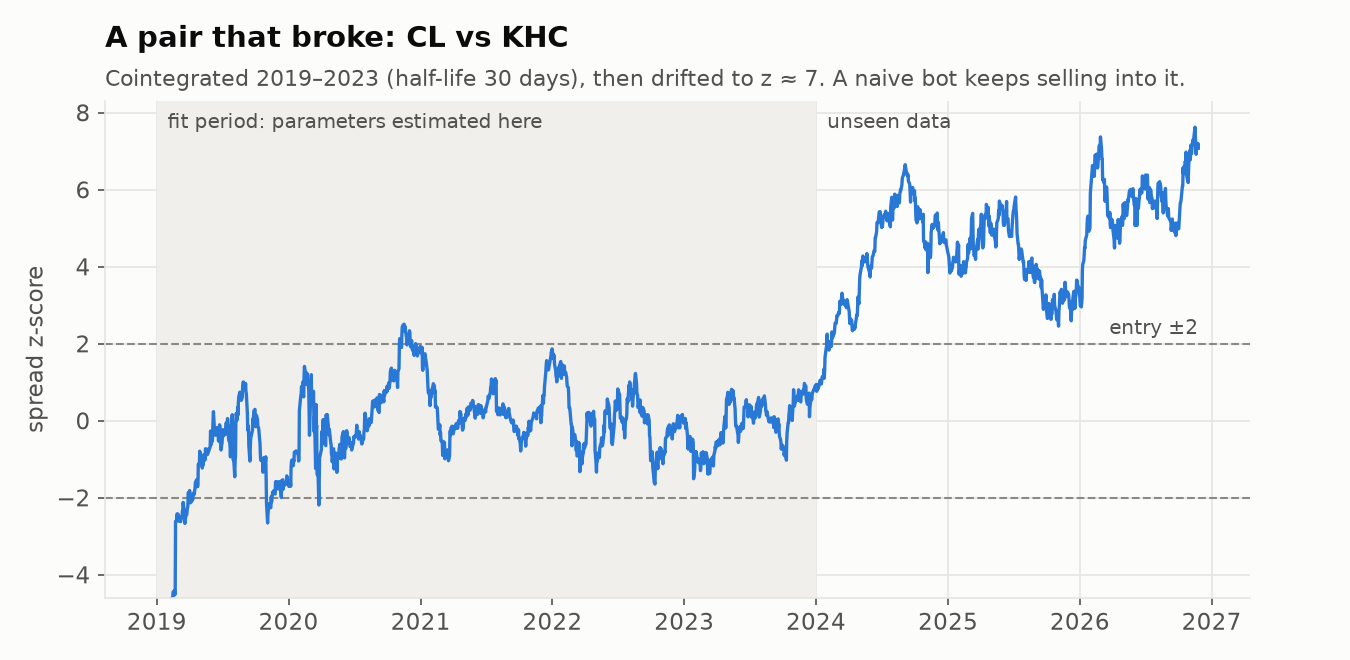
\includegraphics[width=0.92\linewidth]{broken_pair.png}
\caption{Spread z-score of CL versus KHC with parameters frozen at the end of 2023.}
\label{fig:broken}
\end{figure}

\subsection{Walk-forward: cointegration selection}

Across six universes and eight yearly screens, 8{,}672 pair-years were tested
(Figure~\ref{fig:funnel}). 562 (6.5\%) were significant at $p<0.05$ before correction, against
about 434 (5\%) expected if no pair were real. After Benjamini--Hochberg, 21 remained, and
1 also held up in its validation year. That one pair traded twice in eight years. The
thresholds were not loosened to produce trades.

\begin{figure}[ht]
\centering
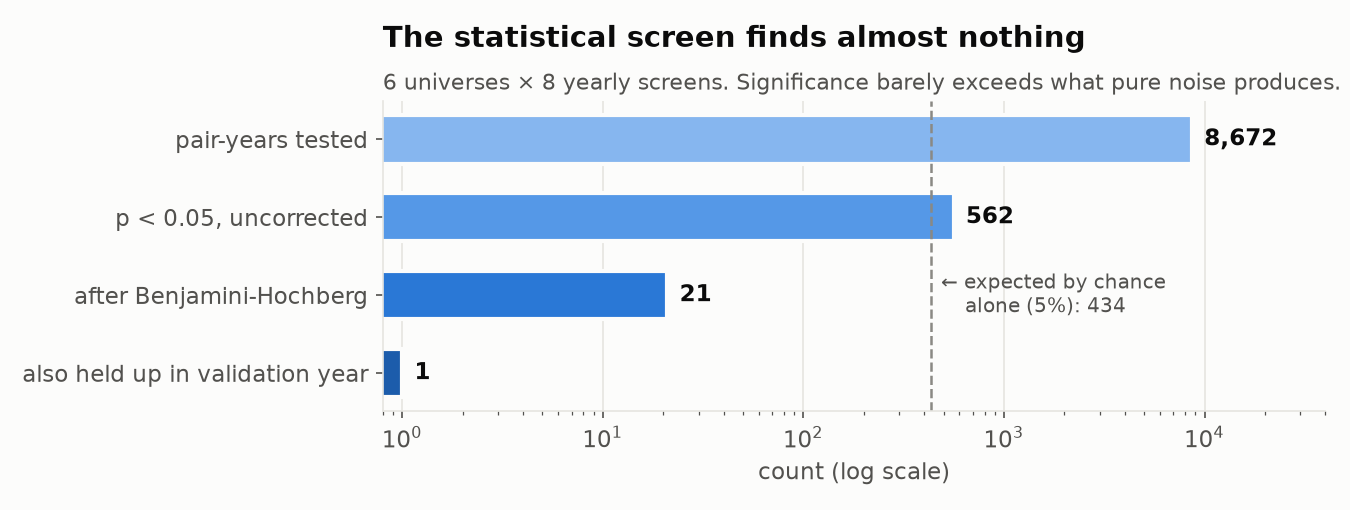
\includegraphics[width=0.92\linewidth]{screen_funnel.png}
\caption{Screening funnel across 6 universes $\times$ 8 years (log scale).}
\label{fig:funnel}
\end{figure}

\subsection{Walk-forward: distance method}

The distance method trades frequently but earns nothing (Table~\ref{tab:dist},
Figure~\ref{fig:equity}).

\begin{table}[ht]
\centering
\caption{Distance-method walk-forward results, 2019--2026. Sharpe ratios are annualized.}
\label{tab:dist}
\begin{tabular}{lrrrr}
\toprule
Universe & Sharpe, 0 bp & Sharpe, 5 bp & Sharpe, 20 bp & Trades\\
\midrule
Banks         & $+0.16$ & $-0.08$ & $-0.82$ & 259\\
Utilities     & $-0.24$ & $-0.60$ & $-1.67$ & 290\\
Energy        & $+0.32$ & $+0.19$ & $-0.20$ & 215\\
REITs         & $-0.04$ & $-0.34$ & $-1.21$ & 221\\
Staples       & $-0.01$ & $-0.20$ & $-0.80$ & 247\\
Country ETFs  & $-0.07$ & $-0.48$ & $-1.67$ & 277\\
\midrule
All 6 combined & $+0.16$ ($t=0.46$) & $-0.41$ ($t=-1.16$) & & 1{,}509\\
\bottomrule
\end{tabular}
\end{table}

\begin{figure}[ht]
\centering
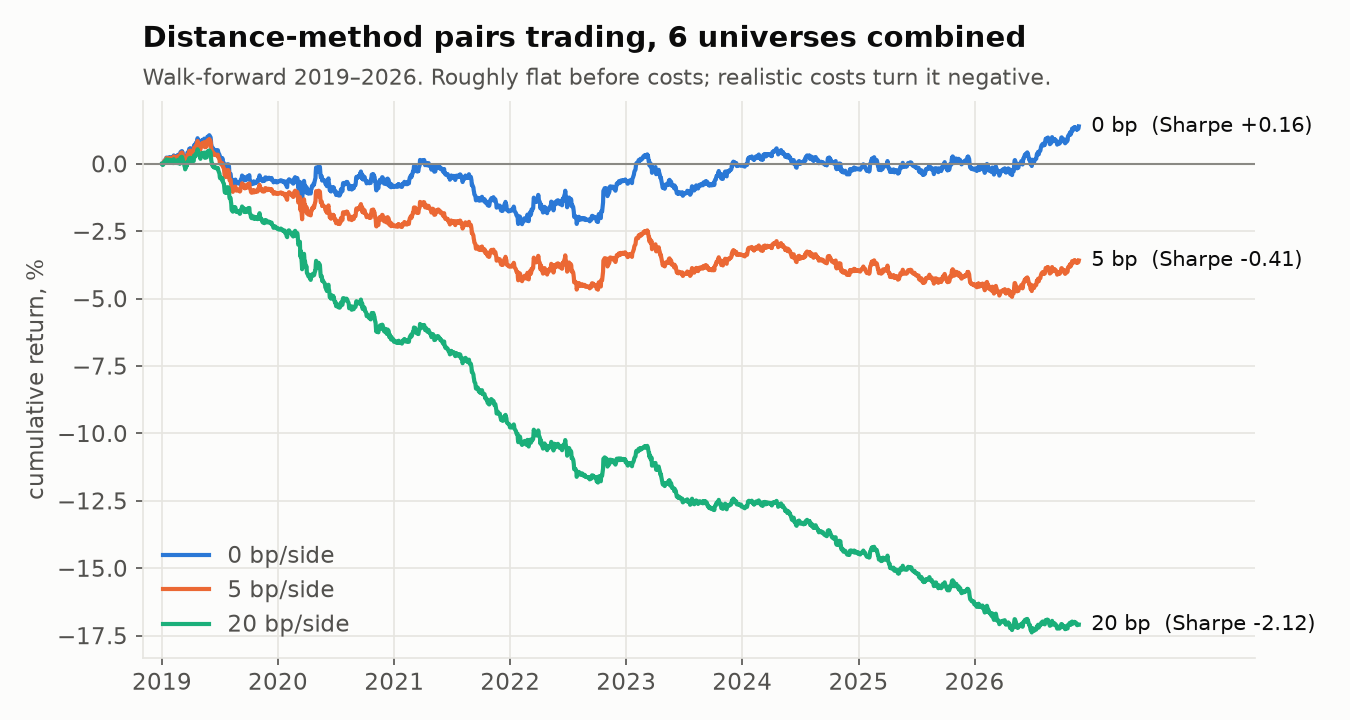
\includegraphics[width=0.92\linewidth]{equity_curves.png}
\caption{Cumulative return of the distance method, six universes combined, at 0, 5 and
20 basis points per side.}
\label{fig:equity}
\end{figure}

The best single result (energy, $+0.19$ after costs) is the best of six tries with
$t\approx0.5$ and is not evidence of an edge. The anatomy of the trades explains the loss:
817 of 1{,}509 trades hit the stop-loss, averaging $-1.2\%$. Trades that do revert earn
$+2.8\%$ on average, but there are too few of them. The spread usually keeps widening instead
of reverting, consistent with \citet{do2010}.

\section{Discussion}

Three lessons stand out. First, multiple testing dominates: the raw rate of ``significant''
pairs is barely above what noise produces, so any strategy that trades uncorrected
significance is mostly trading noise. Second, relationships break: in-sample cointegration
is weak evidence about the future, and pairs in this period were exposed to regime changes
(the 2020 pandemic shock and the 2022--2023 rate cycle). Third, model flexibility must be
checked against noise: two widely used Kalman setups manufacture pairs, and the fix is to
evaluate the tradeable portfolio rather than an internal filter quantity.

A Sharpe ratio estimated over about eight years has a standard error of roughly
$1/\sqrt{8}\approx0.35$, so $t\approx \text{SR}\sqrt{T}$. The pre-cost Sharpe of $+0.16$ is
statistically indistinguishable from zero, and costs of a few basis points are enough to make
it negative. Consistent with the project's plan, no strategy was promoted to paper trading.

\section{Limitations}

\begin{itemize}
  \item \textbf{Survivorship bias:} universes exclude delisted and acquired firms.
  \item \textbf{Two-asset relationships only:} Engle--Granger assumes one cointegrating vector;
        baskets would require the Johansen procedure \citep{johansen1988}.
  \item \textbf{Kalman power loss:} with stable hedge ratios the Kalman screen finds fewer real
        pairs (11/18 versus 18/18).
  \item \textbf{ADF over-rejection:} when a random walk carries large stationary noise,
        ADF can over-reject \citep{schwert1989}; the out-of-sample half-life check catches most
        such cases.
  \item \textbf{Execution simplifications:} daily closes only, uncharged daily rebalancing,
        zero return on idle cash, and no short-sale availability constraints.
  \item \textbf{Researcher degrees of freedom:} although rules were fixed in advance, design
        choices (universes, windows, the trend term) were still made by a person who saw some
        data. The trend term was tuned on a control pair to limit this.
\end{itemize}

\section{Further questions}

The results raise several questions this project does not answer.

\begin{enumerate}
  \item \textbf{Is the null result specific to liquid US equities?} Small caps, non-US markets,
        and less efficient asset classes have fewer arbitrageurs. Does mean reversion survive
        costs there, once those markets' higher costs are included?
  \item \textbf{How much statistical power does the holdout test have?} A planted pair with a
        6-day half-life failed ADF on 190 days. What holdout length is needed to detect a pair
        with a given half-life and spread volatility at 80\% power, and how does that trade off
        against the risk that the relationship decays during a longer holdout?
  \item \textbf{Can a pair's breakdown be detected before the stop-loss?} More than half of
        distance-method trades exited at $|z|>4$. Could structural-break tests (e.g.\ CUSUM on
        the spread) or a rolling half-life exit earlier and cut the average loss?
  \item \textbf{Are there regimes in which pairs revert?} Does profitability depend on market
        volatility, interest-rate regimes, or dispersion across stocks? Any such conditioning
        must be specified in advance to avoid another layer of multiple testing.
  \item \textbf{How many effective trials were run?} Counting all design variants explored,
        what is the deflated Sharpe ratio \citep{bailey2014} of the best configuration, and
        does any result survive the higher hurdle suggested by \citet{harvey2016}?
  \item \textbf{Can the Kalman screen recover its lost power?} Would a likelihood-ratio test of
        $q=0$ (choosing the static model when $\beta$ does not drift), or an informative prior
        on $q$, match the static screen's 18/18 while keeping the gains under drift?
  \item \textbf{Is the GLD/IAU candidate tradeable?} Its spread is driven by a fee difference
        and is very small. Is its volatility large enough relative to bid-ask costs to earn
        anything at all?
  \item \textbf{Does higher frequency change the picture?} Intraday spreads may revert in
        minutes rather than days. Would intraday data reveal mean reversion that daily closes
        miss, and would it survive intraday costs?
  \item \textbf{Is linear cointegration the right model?} Alternatives include fractional
        cointegration, copula-based dependence, and baskets of more than two securities.
\end{enumerate}

\section{Next steps}

Table~\ref{tab:next} lists concrete next steps in priority order, each with the criterion that
would mark it done.

\begin{table}[ht]
\centering
\caption{Roadmap.}
\label{tab:next}
\small
\begin{tabular}{p{0.04\linewidth}p{0.30\linewidth}p{0.56\linewidth}}
\toprule
\# & Step & Done when\\
\midrule
1 & Pre-register the next test & A dated file in the repository fixes universes, windows,
    rules, costs and the success threshold before any new data are examined.\\
2 & Remove survivorship bias & Universes are rebuilt point-in-time from a data source that
    includes delisted securities, and the Stage~3 results are rerun.\\
3 & Power analysis & A simulation table gives detection rates by half-life, spread
    volatility and holdout length, and the holdout length is chosen from it.\\
4 & Johansen baskets & A basket screen with the same FDR control and frozen holdout test
    passes the synthetic ground-truth tests.\\
5 & Better cost model & Rebalancing costs are charged, short-borrow availability is checked
    (e.g.\ Alpaca's shortable and easy-to-borrow flags), and costs are estimated from quotes.\\
6 & New universes & Small caps, international ETFs, and ETF-versus-constituent pairs are
    screened with the same pipeline.\\
7 & Deflated Sharpe & Every reported result includes a deflated Sharpe ratio based on the
    number of configurations tried.\\
8 & Stage 4 gate & Paper trading on Alpaca starts only if a pre-registered walk-forward test
    shows Sharpe above a stated threshold with $t>2$ after 5 bp costs; it then runs at least
    six months, comparing paper fills with backtest assumptions.\\
\bottomrule
\end{tabular}
\end{table}

\section{Conclusion}

After realistic costs, neither a statistically screened cointegration strategy nor the
classic distance method made money on about 120 liquid US stocks and ETFs from 2019 to 2026.
The pipeline finds planted pairs in synthetic data and profits from them, so this conclusion
concerns the market rather than the code. The project's main value is methodological:
correcting for multiple testing, validating on frozen out-of-sample data, testing adaptive
models against pure noise, and declining to trade a strategy the evidence does not support.

\appendix
\section{Reproducibility}

The code is about 1{,}500 lines of Python. Sixteen unit tests run on synthetic data and need
no API keys; continuous integration runs them on every push.

\begin{table}[ht]
\centering
\small
\begin{tabular}{ll}
\toprule
File & Purpose\\
\midrule
\code{src/data.py} & Alpaca daily closes, adjusted and cached\\
\code{src/universes.py} & Sector universes\\
\code{src/synthetic.py} & Synthetic markets with planted pairs\\
\code{src/ou.py} & OU estimation and simulation\\
\code{src/screen.py} & Stage 1 and Stage 2 screens, Benjamini--Hochberg\\
\code{src/kalman.py} & Kalman filter and maximum-likelihood fit\\
\code{src/backtest.py} & Trading rules, walk-forward loop, performance\\
\code{run\_screen.py}, \code{run\_backtest.py} & Command-line entry points\\
\code{make\_figures.py} & Figures in this paper\\
\bottomrule
\end{tabular}
\end{table}

\noindent Typical commands:
\begin{verbatim}
python -m pytest
python run_screen.py --demo
python run_screen.py --universe staples --method kalman
python run_backtest.py --universe all --select coint distance --costs 0 5 10 20
python make_figures.py
\end{verbatim}

\begin{thebibliography}{99}

\bibitem[Bailey and L\'opez de Prado(2014)]{bailey2014}
Bailey, D.~H. and L\'opez de Prado, M. (2014).
The deflated Sharpe ratio: correcting for selection bias, backtest overfitting, and
non-normality. \emph{Journal of Portfolio Management}, 40(5), 94--107.

\bibitem[Benjamini and Hochberg(1995)]{benjamini1995}
Benjamini, Y. and Hochberg, Y. (1995).
Controlling the false discovery rate: a practical and powerful approach to multiple testing.
\emph{Journal of the Royal Statistical Society, Series B}, 57(1), 289--300.

\bibitem[Dickey and Fuller(1979)]{dickey1979}
Dickey, D.~A. and Fuller, W.~A. (1979).
Distribution of the estimators for autoregressive time series with a unit root.
\emph{Journal of the American Statistical Association}, 74(366), 427--431.

\bibitem[Do and Faff(2010)]{do2010}
Do, B. and Faff, R. (2010).
Does simple pairs trading still work? \emph{Financial Analysts Journal}, 66(4), 83--95.

\bibitem[Elliott et~al.(2005)]{elliott2005}
Elliott, R.~J., van der Hoek, J. and Malcolm, W.~P. (2005).
Pairs trading. \emph{Quantitative Finance}, 5(3), 271--276.

\bibitem[Engle and Granger(1987)]{engle1987}
Engle, R.~F. and Granger, C.~W.~J. (1987).
Co-integration and error correction: representation, estimation, and testing.
\emph{Econometrica}, 55(2), 251--276.

\bibitem[Gatev et~al.(2006)]{gatev2006}
Gatev, E., Goetzmann, W.~N. and Rouwenhorst, K.~G. (2006).
Pairs trading: performance of a relative-value arbitrage rule.
\emph{Review of Financial Studies}, 19(3), 797--827.

\bibitem[Harvey et~al.(2016)]{harvey2016}
Harvey, C.~R., Liu, Y. and Zhu, H. (2016).
\ldots{} and the cross-section of expected returns.
\emph{Review of Financial Studies}, 29(1), 5--68.

\bibitem[Johansen(1988)]{johansen1988}
Johansen, S. (1988).
Statistical analysis of cointegration vectors.
\emph{Journal of Economic Dynamics and Control}, 12(2--3), 231--254.

\bibitem[Kalman(1960)]{kalman1960}
Kalman, R.~E. (1960).
A new approach to linear filtering and prediction problems.
\emph{Journal of Basic Engineering}, 82(1), 35--45.

\bibitem[Schwert(1989)]{schwert1989}
Schwert, G.~W. (1989).
Tests for unit roots: a Monte Carlo investigation.
\emph{Journal of Business \& Economic Statistics}, 7(2), 147--159.

\bibitem[Uhlenbeck and Ornstein(1930)]{uhlenbeck1930}
Uhlenbeck, G.~E. and Ornstein, L.~S. (1930).
On the theory of the Brownian motion. \emph{Physical Review}, 36(5), 823--841.

\bibitem[Vidyamurthy(2004)]{vidyamurthy2004}
Vidyamurthy, G. (2004).
\emph{Pairs Trading: Quantitative Methods and Analysis}. Wiley.

\end{thebibliography}

\end{document}
